\documentclass[11pt,a4paper]{article}
\usepackage[margin=19mm,headheight=15pt,footskip=11mm]{geometry}
\usepackage[T1]{fontenc}
\usepackage{lmodern,amsmath,amssymb,graphicx,booktabs,array,tabularx,xcolor}
\usepackage{tikz}
\usetikzlibrary{arrows.meta,positioning,fit}
\usepackage{caption,fancyhdr,hyperref,url,xurl}
\setlength{\emergencystretch}{3em}
\definecolor{navy}{HTML}{245B89}
\definecolor{teal}{HTML}{24836B}
\definecolor{rust}{HTML}{B54B4B}
\hypersetup{colorlinks=true,linkcolor=navy,urlcolor=navy,citecolor=navy,pdftitle={Reinforcement Learning for Prince Valiant: A Case Study},pdfauthor={Orkun Taha Öznergiz}}
\urlstyle{tt}
\setlength{\parindent}{0pt}
\setlength{\parskip}{5pt plus 1pt}
\setlength{\tabcolsep}{4pt}
\renewcommand{\arraystretch}{1.14}
\newcolumntype{Y}{>{\raggedright\arraybackslash}X}
\newcolumntype{P}[1]{>{\raggedright\arraybackslash}p{#1}}
\captionsetup{font=small,labelfont=bf,skip=5pt}
\pagestyle{fancy}\fancyhf{}
\fancyhead[L]{\small\textcolor{navy}{PRINCE VALIANT / LEARNING FROM RAM}}
\fancyhead[R]{\small Case study / 26 October 2026}
\fancyfoot[L]{\small Orkun Taha Öznergiz}
\fancyfoot[R]{\thepage}
\newcommand{\topic}[2]{\vspace*{-4mm}{\small\color{teal}\textbf{#1}}\par{\LARGE\bfseries #2}\par\vspace{3mm}}
\newcommand{\ev}[1]{{\small\textcolor{navy}{[#1]}}}
\newcommand{\pathref}[1]{\nolinkurl{#1}}
\newcommand{\fig}[4]{\begin{figure}[ht]\centering\includegraphics[width=#2\linewidth]{assets/#1}\caption{#3}\label{#4}\end{figure}}
\tikzset{box/.style={draw=navy,rounded corners,fill=navy!5,align=center,font=\small,minimum height=11mm},arr/.style={-{Latex[length=2mm]},thick,navy}}
\begin{document}
\topic{01 / PROJECT OVERVIEW}{Reinforcement Learning for Prince Valiant}
{\large RAM instrumentation, reinforcement learning, and route imitation}\par
\textbf{Orkun Taha Öznergiz}\hfill 26 October 2026

I developed a learning system for \emph{The Legend of Prince Valiant}: an emulator interface, RAM observations, human-play recording, neural controllers, and tools to verify their gameplay. I supplied the human demonstrations and directed the project's goals and iterations. AI coding assistance supported implementation and documentation; the underlying NES emulator and machine-learning libraries are existing dependencies.

The approach changed with the results. PPO exposed coverage and control problems. Demonstration-assisted Q-learning produced the selected Level~1 clear; local Level~2 skills did not reliably compose into a route, so the final later-level policies use imitation. Separate models and saved starting states are used.

\begin{table}[ht]\centering\small
\begin{tabularx}{\linewidth}{@{}P{12mm}P{29mm}P{33mm}Y@{}}\toprule
Level & Selected policy & Reviewed run / start & Demonstrated result and acceptance gap\\\midrule
1 & DQN/DQfD update3,000 & One greedy episode; reset389 & Clear in 18,273 frames, return 108.091791. Normal-start compliance unaudited.\\
2 & Title-inclusive imitation & One v59 corroboration; saved title entry & Complete card and Level3 entry. Known training route; reliability unmeasured.\\
3 & Raw-RAM imitation & One v2 run; saved intro state & Complete card and Level4 title. Source-route reproduction; recovery unmeasured.\\\bottomrule
\end{tabularx}
\caption{Selected results. These are not independent ten-episode campaigns. Replays and alternative checkpoints do not increase each selected policy's qualifying trial count. No level's 7/10 requirement is established.}\label{tab:overview}
\end{table}
\begin{figure}[ht]\centering
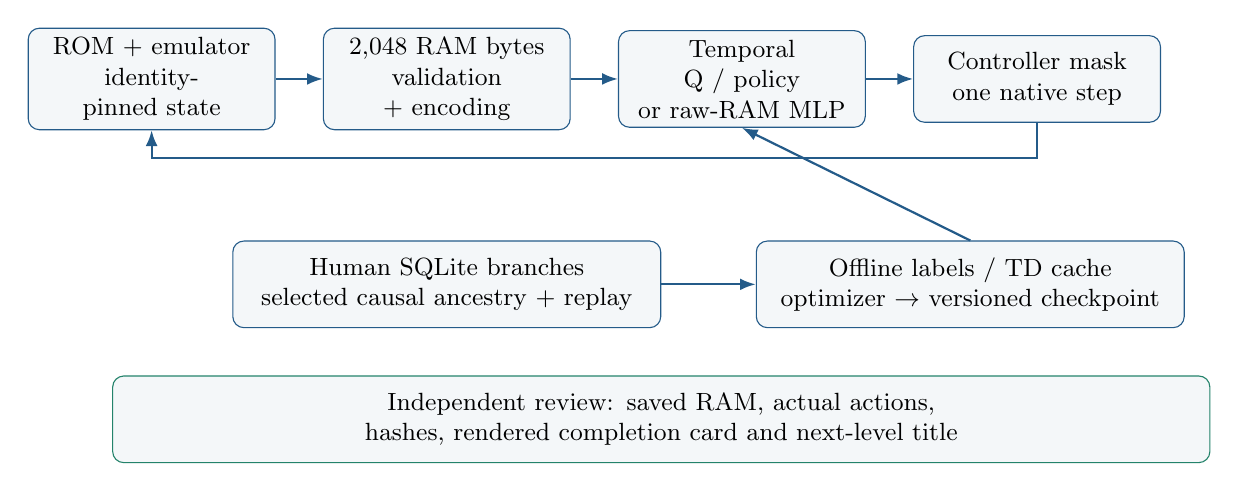
\begin{tikzpicture}[node distance=6mm]
\node[box,text width=29mm] (rom) {ROM + emulator\\identity-pinned state};
\node[box,text width=29mm,right=of rom] (ram) {2,048 RAM bytes\\validation + encoding};
\node[box,text width=29mm,right=of ram] (model) {Temporal Q / policy\\or raw-RAM MLP};
\node[box,text width=29mm,right=of model] (step) {Controller mask\\one native step};
\draw[arr] (rom)--(ram);\draw[arr] (ram)--(model);\draw[arr] (model)--(step);
\draw[arr] (step.south) -- ++(0,-.45) -| (rom.south);
\node[box,text width=52mm,below=14mm of ram] (demo) {Human SQLite branches\\selected causal ancestry + replay};
\node[box,text width=52mm,right=12mm of demo] (train) {Offline labels / TD cache\\optimizer $\to$ versioned checkpoint};
\draw[arr] (demo)--(train);\draw[arr] (train.north)--(model.south);
\node[box,draw=teal,text width=137mm,below=6mm of demo.south east,anchor=north] (review) {Independent review: saved RAM, actual actions, hashes, rendered completion card and next-level title};
\end{tikzpicture}
\caption{Implemented paths. Inference acts through ordinary controller input; demonstration processing and optimization are separate. The reviewer corroborates the resulting trajectory.}\label{fig:pipeline}
\end{figure}

The case study follows the implementation decisions, measured failures and retained solutions. Appendix references and the evidence ledger identify the supporting artifacts. No new training or gameplay was run for this revision. \ev{E01--E26}

\newpage
\topic{02 / MEASUREMENT}{RAM semantics require experiments}
\textbf{Native contract.} \pathref{RecorderNative} wraps a C ABI through \pathref{ctypes}. A controller mask advances one native frame; RAM is exposed as 2,048 \pathref{uint8} bytes and copied before subsequent mutation. Masks encode A=1, B=2, SELECT=4, START=8, UP=16, DOWN=32, LEFT=64 and RIGHT=128. Selected Level~1 inference uses 17 masks and frame skip~1. Native frames, decisions, optimizer updates, and wall seconds remain distinct units. The emulator's 60-frame convention converts simulated time; the ROM's PAL label alone does not set measured timing. \ev{E01,E02}

Full states include CPU/emulator/mapper state, rather than RAM alone. The \pathref{PVSTATE1} envelope validates ROM hash, native build identity and payload SHA-256. Restoration uses a fresh native owner so rejection cannot corrupt the existing game. A compatible RAM vector alone cannot guarantee a compatible future trajectory. Recorded pre/post RAM and actual control histories support deterministic replay; loaded framebuffer composition can nevertheless be stale. \ev{E01}

\textbf{Semantic investigation.} A byte correlation generates a hypothesis. Executed 6502 instructions, bank-aware ROM context and bus writes identify the computation; paired controls test a scoped mechanism; rendered evidence checks its game meaning. Three examples illustrate the distinction:

\begin{tabularx}{\linewidth}{@{}P{27mm}Y Y@{}}\toprule
Example & Verified mechanism & Boundary of inference\\\midrule
Rope attachment & Bank~7 \texttt{\$EA16--EA9D} uses selected slot \texttt{\$2F2}, segment \texttt{\$2F3}, and ROM pose table \texttt{\$EA9E}. Fixed anchor coordinates do not describe the moving attachment. & Slot/segment bytes persist after release; interpretation requires player state~23 and valid type/geometry.\\
Player extents & \texttt{\$63} selects paired data; \texttt{\$D173--D17E} writes comparison extents \texttt{\$68/69}; overlap/probe routines consume them. & Comparison extents and sprite drawing rectangles do not certify a universal collision hitbox.\\
Level~2 drop dispatch & Saved failed frame~17239 loads projectile status~1 and returns; successful frame~4740 loads~129 and reaches the guarded award path. 129 replay frames match all RAM bytes. & Two trajectories do not establish a universal collision or spawn rule.\\\bottomrule
\end{tabularx}
\ev{E08,E14; exact primary trace locations in Appendix B}

\textbf{Rewind ancestry.} SQLite stores executed inputs, pre/post RAM, full checkpoints, and branch ancestry. Restoring a checkpoint creates a branch. Appending the abandoned future to its replacement would invent a causal transition and contaminate TD targets. Selected ancestry cuts each parent at the restored checkpoint; continuity requires the next pre-RAM to equal the preceding post-RAM.

\begin{figure}[ht]\centering
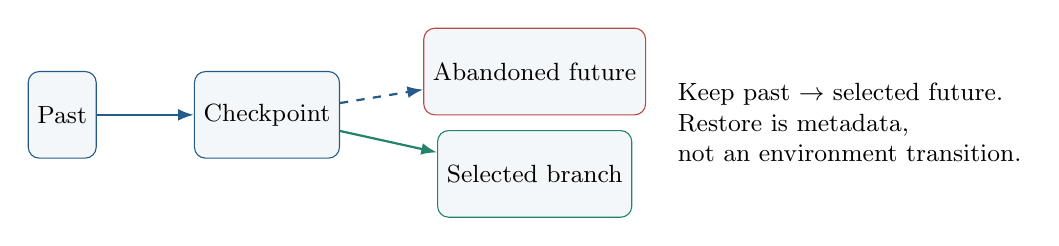
\begin{tikzpicture}[x=1cm,y=1cm]
\node[box] (a) at (0,0) {Past};\node[box] (b) at (2.6,0) {Checkpoint};
\node[box,draw=rust] (c) at (6,0.55) {Abandoned future};
\node[box,draw=teal] (d) at (6,-.75) {Selected branch};
\draw[arr] (a)--(b);\draw[arr,dashed] (b)--(c);\draw[arr,teal] (b)--(d);
\node[align=left,font=\small] at (10,-.1) {Keep past $\to$ selected future.\\Restore is metadata,\\not an environment transition.};
\end{tikzpicture}
\caption{Causal ancestry, not recording order, defines the training sequence. Native state/history reconstruct reset context; checkpoint and branch IDs are excluded from policy input.}\label{fig:ancestry}
\end{figure}

\newpage
\topic{03 / REPRESENTATION}{Versioned observations and neural structure}
\textbf{Why RAM and history?} RAM exposes compact numeric state without first solving image recognition, making feature extraction and replay comparisons practical. It still omits CPU/mapper state and can hide motion, input edges and context from a single observation. A finite history helps resolve those control ambiguities; opaque raw bytes can also encode route-specific timing, which limits generalization.

Let $x_t\in\{0,\ldots,255\}^{2048}$ denote current RAM, $a_t$ the executed action, and $v_t$ availability masks. For selected Level~1, $o_t=E(x_{\le t},a_{<t};v_t)$ is an engineered observation. Its fixed window is
\begin{equation}\label{eq:window}
 W_t=(o_{t+\delta},v_{t+\delta})_{\delta\in\{-60,-30,-15,-9,-6,-3,0\}},\quad
 z_t=\operatorname{GRU}_{h_0=0}(F(W_t))_{\rm last}.
\end{equation}
History is measured in native frames, not adjacent decisions when held actions are used. The selected reset-389 receipt has only its current slot valid and six past slots invalid; it must not be described as a fully warm seven-frame reset. Other earlier-start studies reconstruct genuine prehistory. Previous actual masks and press/release ages, capped at 120 frames with separate validity, describe control edges. \ev{E02,E06}

\begin{tabularx}{\linewidth}{@{}P{37mm}Y@{}}\toprule
Input group & Role in the selected Level1 controller\\\midrule
Player, camera and controls & Position/resources, actual past masks, button-edge ages and validity\\
Object and projectile records & Masked relative geometry, raw state codes and conservative motion continuity\\
Terrain and moving geometry & $12\times17$ grids for collision classes, actors and rope attachment points\\
Triggers and resident records & Scoped ROM/RAM context with explicit availability\\\bottomrule
\end{tabularx}
The exact tensor dimensions and schema are retained in Appendix~F.

The seven offsets span one second at the emulator's 60-frame convention: older samples supply context, while denser recent samples preserve action timing. This is the selected design, not an ablation-proven optimum. The same encoders process each timestamp. Structured features and terrain/motion CNN features are combined, then a GRU summarizes the ordered window. Resetting its hidden state makes each replayed window self-contained and reproducible across shuffled training batches. A persistent recurrent state would need a different sequence/replay contract; no superiority comparison was run. \ev{E06}

\begin{figure}[ht]\centering
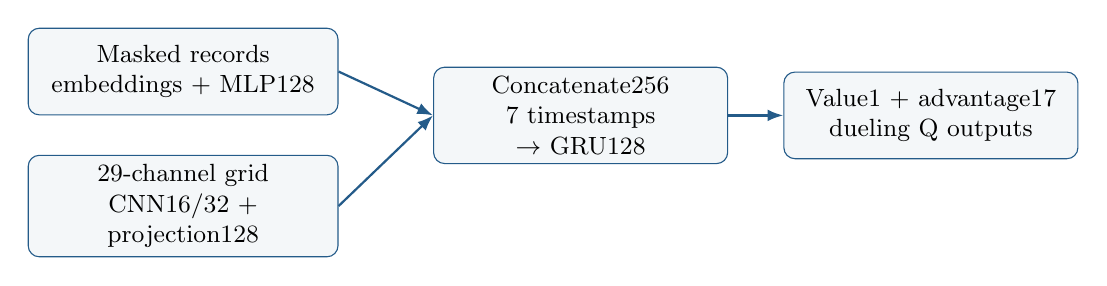
\begin{tikzpicture}[node distance=7mm]
\node[box,text width=37mm] (s) {Masked records\\embeddings + MLP128};
\node[box,text width=37mm,below=5mm of s] (g) {29-channel grid\\CNN16/32 + projection128};
\node[box,text width=35mm,right=12mm of s.south east,anchor=west] (f) {Concatenate256\\7 timestamps $\to$ GRU128};
\node[box,text width=35mm,right=of f] (q) {Value1 + advantage17\\dueling Q outputs};
\draw[arr] (s.east)--(f.west);\draw[arr] (g.east)--(f.west);\draw[arr] (f)--(q);
\end{tikzpicture}
\caption{Selected DQfD online network (1,234,458 parameters); a separate target copy supplies bootstrap values. The earlier PPO family has independent actor and critic encoders, not these dueling output heads. Initial DQN transfer uses only the earlier BC actor encoder; its action-logit head is excluded.}\label{fig:model}
\end{figure}

Level~2's final imitation actor instead uses $2048\to256\to128\to16$ (559,504 parameters). Level~3 independently uses $2048\to512\to256\to22$ (1,186,070). Their inputs are opaque current RAM with embedded mean/scale normalization; neither is this structured temporal schema. Exact raw controller vocabularies differ by level. \ev{E17,E19}

\newpage
\topic{04 / LEARNING OBJECTIVES}{Demonstration-assisted TD is distinct from cloning}
\textbf{Selected Level~1 objective.} Dueling Q-learning estimates
\[Q_\theta(W,a)=V_\theta(z)+A_\theta(z,a)-|\mathcal A|^{-1}\sum_b A_\theta(z,b).\]
Here $r_i$ is transition reward, $d_i$ its native-frame duration, $b_i$ the bootstrap flag, and $D_k=\sum_{j=0}^{k-1}d_{i+j}$. Targets combine recorded rewards with the target network estimate:
\begin{align}
 R_i^{(n)}&=\sum_{k=0}^{n-1}\gamma^{D_k}r_{i+k},\quad \Gamma_i^{(n)}=\gamma^{D_n},\label{eq:return}\\
 y_i^{(n)}&=R_i^{(n)}+b_i^{(n)}\Gamma_i^{(n)}
 Q_{\bar\theta}\!\left(W_{i+n},\arg\max_{a\in\mathcal A_i}Q_\theta(W_{i+n},a)\right).\label{eq:target}
\end{align}
The paired-return helper shortens at boundaries without joining owners/episodes. Natural game-over/completion and unsupported states disable bootstrap; a time limit retains the actual continuation. Training life-loss truncation, when enabled, has a distinct bootstrap-valid contract. Death is not automatically game-over. The selected skip-1 continuation has $d_i=1$. \ev{E04,E07}

Writing $\rho$ for smooth-L1 (Huber), $m=0.8$, and $q_i=Q_\theta(W_i,a_i)$, the \emph{implemented} batch objective is
\begin{align}
 M_i&=\max_{a\in\mathcal A_i}\{Q_\theta(W_i,a)+m\mathbf1[a\ne a_i]\}-q_i,\\
 \mathcal L_{\rm DQfD}&=\frac1B\sum_i w_i\!\left[\rho(q_i-y_i^{(1)})+\rho(q_i-y_i^{(10)})+
 \mathbf1_{\rm demo}M_i\right]+10^{-5}\!\sum_{p\in\theta}\|p\|_2^2.\label{eq:dqfd}
\end{align}
All three row terms have coefficient~1 and receive importance weights; the L2 term is applied once per batch. It is verified in this implementation, rather than inferred from the algorithm name. Online Q selects the next action; detached target Q evaluates it (Double DQN). The helper supports masks; all 17 selected gameplay actions are legal. \ev{E04,E05} The method follows DQfD and Double-Q principles \cite{dqfd,doubleq}, but the successful continuation uses demonstrations only.

\textbf{Why these losses?} One-step TD learns immediate consequences, ten-step TD carries later rewards back through a short sequence, and the demonstration margin protects recorded actions from being outranked without evidence. Prioritized replay revisits high-error examples. This does not guarantee retained gameplay: the later checkpoint regression is a direct counterexample. The exact replay distribution, importance weights, optimizer and restoration settings are listed in Appendix~F. \ev{E04,E05}

\textbf{Cloning.} For Levels~2/3, ordinary action supervision minimizes
\begin{equation}\label{eq:bc}
 \mathcal L_{\rm BC}=-\frac1B\sum_i\log \pi_\theta(a_i\mid\tilde x_i),\qquad
 \tilde x_j=\frac{x_j/255-\mu_j}{\max(\sigma_j,0.02)}.
\end{equation}
No environment reward is optimized in those fitting stages. Hard-example sampling changes which recorded rows are fitted; it does not create independent experience. \ev{E17,E19--E21}

\newpage
\topic{05 / CURRICULA AND REWARDS}{Control exposure before interpreting learning}
\textbf{Train the ending, then expand coverage.} Backward curricula first expose a short demonstrated suffix, then move the start earlier after enough successful rollouts. Dedicated full-start, coverage and frontier/rehearsal collectors prevent one start type from consuming all experience; only frontier outcomes advance its stage. The exact settings changed between versions, so configured stages are not treated as demonstrated mastery.

Training resets reconstruct legitimate history and seed previously earned progress without paying it again. Curriculum IDs and future demonstration actions are excluded from policy input. Evaluation retains normal lives and respawns. Diagnostic enemy removal or damage guards belong to controlled studies, not the reported clear runs. \ev{E02,E07}

\textbf{Reward versions.} The selected Level~1 continuation retains \texttt{level1\_phase\_corridor\_v6}, inherited from its config lineage. Table~\ref{tab:rewards} lists every configured coefficient. Coefficients multiply events with different scales; their magnitudes are not comparable contributions. Appendix~A gives event definitions, availability and safeguards. \ev{E02,E07}

\begin{table}[ht]\centering\small
\begin{tabular}{@{}lr lr@{}}\toprule
Level~1 term & Weight & Level~1 term & Weight\\\midrule
First progress /16 pixels & $+0.2$ & Player HP-loss fraction & $-2$\\
First section/checkpoint & $+2$ & Death started & $-2$\\
First cleared objective & $+3$ & Lives lost & $-4$\\
Verified level completion & $+40$ & Game-over event & $-4$\\
Route corridor difference & $+2$ & Elapsed seconds & $-0.03$\\
Combat potential difference & $+6$ & Enemy damage & $0$\\
Verified enemy defeats & $+0.25$ & ABI2 kind18 defeat & $0$\\
Valid displayed-score gain & $+0.00005$ & &\\\bottomrule
\end{tabular}
\caption{Selected Level~1 weights. A zero coefficient does not certify availability of the corresponding semantic event.}\label{tab:rewards}
\end{table}

The potential terms are implemented differences of the form
\begin{equation}\label{eq:potential}
 F_t=\gamma\,b_t\Phi(x_{t+1})-\Phi(x_t),\qquad r_t=\sum_k c_k e_{k,t}.
\end{equation}
Progress/objective memory blocks repeated payouts, score decoding rejects unsupported changes, and unavailable damage is kept distinct from zero. These checks reduce obvious farming opportunities; they do not prove the reward is optimally balanced. Potential differences are scoped to the implemented termination/history contract, without a blanket policy-invariance claim.

\textbf{What actually contributed?} On the saved clear training trace, progress contributes 59.69, completion 40, objectives 12 and time$-9.14$; score contributes only 0.57. A failed PPO suffix instead accumulates life/death/game-over costs totaling$-32$. Appendix~F lists complete component totals and their differing starts; this is descriptive, not an algorithm comparison or trained reward ablation. With $\gamma=0.99997$, reward weight falls to$e^{-1}$ after about 33,333 native frames (556 simulated seconds), longer than the 18,273-frame clear. This is a discount timescale, not the collection horizon. Changed reward coefficients require consistent one-/ten-step replay relabeling; the successful continuation held them fixed.

Level~2 v3 uses completion $+100$, game over $-25$, ENERGY-loss fraction $-5$, and seconds $-0.01$; v4 adds displayed score $\times0.01$ with kill/progress/shot rewards zero. Later aim/hold studies add potential $\times0.25$ and eligible aiming seconds $\times0.03$. Directions control aim; score is a progress proxy, not a certified kill count. Aim-before-shoot gates, old-enemy rechecks, target selectors, kind-8 drop adapters and later hard-example imitation are distinct curricula. Prepared phase-removal plans must not be reported as executed mastery. \ev{E12--E18}

\newpage
\topic{06 / LEVEL 1}{Select the clear, not the latest checkpoint}
\fig{07_level1_milestones.pdf}{1}{Compatible Level~1 milestone evaluations from reset~389. Points are single greedy episodes, without interpolation or statistical success-rate claims. Update~2,000 is the preserved earlier baseline; 3,000--5,000 are the continuation. Source: E03.}{fig:l1}
\textbf{Decision: continue offline learning with rewards fixed.} The same 21,599 human/policy demonstration transitions underlie this continuation. Updates 3,000 and 4,000 each terminate naturally after 18,273 frames with return 108.091791 and objective IDs 513/514/515/516. The earlier-update tie rule selects 3,000. Update 5,000 instead reaches game over after 27,246 frames, return 6.722021, with only objective~513. Loss medians decline from 0.19436 to 0.16328 across the first/last 100 continuation updates; that decline does not explain or prevent behavioral regression. \ev{E02,E03}

\textbf{Historical distinction.} A prior epoch-400 \emph{supervised actor} in the BC/PPO architecture also completed the route: all eight prescribed full/suffix/recovery assessments succeeded, but only one used the full reset-389 route. Its five fitted sources already total 21,599 rows, including successful PPO-derived recovery traces. Thus DQfD was not the only completing policy, and the selected final DQfD checkpoint is not the earlier actor. Neither record establishes ten qualifying normal-start episodes. \ev{E09}

\textbf{What DQfD did and did not add.} It introduced reward-based one-/ten-step TD targets and a target Q-network while retaining demonstration supervision. Completion under that objective is demonstrated. Because the earlier BC actor already completed with the same demonstration collection, these results do not isolate a benefit from TD learning over BC. A matched initialization/data/reset/budget comparison would be needed.

\textbf{Why the PPO work did not settle the result.} Earlier-start anchored endpoints died after 3,971 and 3,421 frames, while an auxiliary-BC comparison stopped on host-memory allocations before its scheduled evaluations. Those are different findings: limited control transfer versus incomplete execution. PPO also produced successful local recovery traces, so it is inaccurate to call every PPO run a failure. Appendix~C separates observations, hypotheses and tests; Appendix~F retains the exact run settings.

The observed-evidence/mechanism/alternative/test table is retained in Appendix~C. The anchored earlier-start failures are measured policy outcomes; the allocation-limited auxiliary-BC comparison never reached its scheduled review points.
\smallskip
Long-horizon credit assignment, sparse successful exploration and reward imbalance remain hypotheses where route length and observed coverage make them relevant. No controlled PPO-versus-DQN causal comparison is supported: data, resets, optimization budgets and initialization differ. Startup rejection, storage/report failures and skipped evaluations are kept separate from measured game-over episodes. \ev{E10,E11}

\newpage
\topic{07 / LEVEL 2}{Local skills improved; the route still failed}
\textbf{Problem: sparse useful behavior.} The first resource/control baseline's scratch DQN chose NOOP and died at 6,723 frames. Adding valid score feedback, target-conditioned geometry and an aim-before-shoot curriculum produced a shooter that passed three short encounters. Earlier-start expansion then damaged retained skills. The response was to isolate target selection and add a drop-specific head while freezing established behavior. These were local gains, not a complete route. \ev{E12--E18}

\fig{02_rl_objective_vs_behavior.pdf}{.92}{Expanded drop adapter v33: saved optimizer diagnostics (25-update moving means) versus fresh pickup probes. Six related starts with three timing variants are correlated development cases. Old-enemy probes remained byte-identical 9/9. Source: E12.}{fig:l2loss}

\textbf{Diagnosis: a softer loss did not protect a hard behavior.} The expanded drop head fell from 9/18 to 2/18 source pickups despite preserving old-enemy probes. A later 25-update candidate lost two previously successful timing cases and was rejected. At shared states, fire+right changed to down as the successful action's Q margin crossed zero. TD and geometry gradients opposed rehearsal on the fixed diagnostic dataset. Thus a rehearsal penalty could be outweighed or interfere across states; it was not an action-preservation guarantee. The exact margins, cosines and their noncausal interpretation are retained in Appendix~F. \ev{E13}

\textbf{Response: enforce retention and test transfer.} A saved-action gate accepted one proposal and rejected the next. Motion/dispatch features then improved familiar timing probes from 3/18 to 14/18, but reserved cases changed 1/12 to 0/12. Matched continuous trials collected six drops in each 12-trial arm. These tests did not justify a broader controller promotion. \ev{E14--E16}

\textbf{Decision: fit the continuous route.} Programmed full-route attempts failed; an initial clone also died despite fitting 22,338/22,449 rows. Hard-example refinement completed the gameplay route, and the title-inclusive actor handled entry. Its clear was corroborated with the completion card and next-level transition. Four bonus-priority/fire-fill variants subsequently failed with zero collections, so the existing actor was retained. It collected 7 E and 3 T bonuses while missing 10 of 20 opportunities; pickup control remains incomplete. Version-by-version receipts are in the appendix. \ev{E17,E18}

\newpage
\topic{08 / LEVEL 3}{A neural policy reproduces the demonstrated route}
Level~3 was initialized separately, without transferring Level~1/2 semantic assumptions or weights. The selected ancestry supplies 49,100 training pairs from path frames 44,700--93,800, including intro and transition context. The independent \texttt{level3\_raw\_ram\_imitation\_v1} schema is current $\mathrm{uint8}[2048]$; its MLP has two ReLU hidden layers (512,256), 22 raw-mask logits, and normalization from Equation~\ref{eq:bc}. The dataset contains no conflicting labels for identical RAM rows. Opaque RAM avoids unverified semantic transfer, but counters/context can distinguish positions on this particular route. \ev{E19--E22}

\fig{09_level3_fit_errors.pdf}{.94}{Recorded fitting checkpoints, separated at update20,000. Initial fitting leaves 64 source-action errors; refinement achieves exact 49,100-row agreement in single-row runtime inference. This is training agreement, not held-out accuracy or an RL reward curve.}{fig:l3fit}

\textbf{Problem and response.} The initial 20,000-update supervised fit left 64 incorrect source actions. Low-rate hard-example refinement added 15,500 updates and reached exact single-row agreement. This was an incomplete fit followed by successful refinement, not a failed Level3 RL experiment. Exact fitting makes the known route reproducible; it does not establish recovery from an unfamiliar state. Detailed sampling/rate settings are in Appendix~F. \ev{E20,E21}

\textbf{Closed-loop review.} Observation validation checked 360 native transitions at three anchors. The selected run loads one frame-44700 full state and then makes 49,775 model decisions. Each controller mask is independently recomputed from current RAM and the frozen checkpoint; there is no reference-action lookup, source-frame input, playback cursor, mid-run reset, RAM edit or optimizer during evaluation. \textbf{The first 49,100 reference-range RAM frames match exactly: this is deterministic route reproduction.} A neural controller chooses the actions, but matching the training trajectory leaves recovery and independent-start robustness unmeasured. The 675-frame tail corroborates transition screens, not new-route competence. \ev{E22}

\begin{figure}[ht]\centering

\includegraphics[width=.28\linewidth]{assets/level2_complete.png}\hspace{5mm}

\includegraphics[width=.28\linewidth]{assets/level3_complete.png}\hspace{5mm}
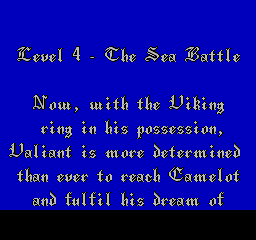
\includegraphics[width=.28\linewidth]{assets/level4_title.png}
\caption{Saved rendered evidence, preserved without regeneration: Level~2 complete at frame 22,809; Level~3 complete at 47,975; Level~4 title at 49,175. Level~2's following title/gameplay occur at 23,409/23,709. Level~3's flag at 47,675 alone was insufficient.}\label{fig:cards}
\end{figure}

Terminal references use active rendering to avoid stale loaded screens. Exact title matching permits only the validated bounded vertical scroll; Appendix~F retains the check. A completion flag or Level4 title alone is not evidence of broader competence. \ev{E18,E22}

\newpage
\topic{09 / REPRODUCIBILITY AND ACCEPTANCE}{What can be reproduced, and what remains open}
\textbf{What a recipient can do today.} Read the code, inspect included checkpoints on CPU after installing dependencies, and review saved plots/videos. A recipient cannot reproduce the selected gameplay runs from the package alone: ROM, reset states, data and compatible native binaries are missing. Current entry points are documented in the package's \pathref{docs/SETUP.md} and \pathref{docs/REPRODUCIBILITY.md}; the internal export handoff has since been consolidated into those guides.

The original export audit checked 246 inventory hashes, import/dependency files and model identities. That dated snapshot is retained separately from subsequent documentation changes; it is not a claim that the current export is unchanged. No clean-machine installation or fresh native gameplay was validated for this case study. \ev{E23,E24}

\begin{tabularx}{\linewidth}{@{}P{31mm}Y P{49mm}@{}}\toprule
Workflow & Review available now & Missing before execution\\\midrule
Checkpoint inspection & CPU model inspector (command in Appendix~G); historical CPU-load check & Install pinned Python dependencies; fresh-machine setup unverified\\
Level1 selected evaluation & Runner, checkpoint and saved receipts & ROM, route/reset389, identity-compatible DLL and ABI2 observer/provenance\\
Level2 confirmed clear & Actor, runner and card/title evidence & ROM, compatible DLL, title/reset/preparation assets\\
Level3 play and review & Actor and recomputation reviewer & ROM/DLL, intro reset/preparation; reviewer also needs reference dataset/images\\\bottomrule
\end{tabularx}
Evaluation commands and exact missing-input families are in Appendix~G. Original-owner restoration can supply private files subject to access/redistribution review; it does not resolve native license provenance or prove a new build compatible. Historical DQfD training receipts cannot authorize a fresh training launch.

\textbf{Acceptance still pending.} None of the selected levels has the required 7/10 campaign, and Level1 normal-start compliance remains unaudited (Table~\ref{tab:overview}). The full requirement/evidence/gap table is retained in Appendix~G. More complex models do not close these evaluation gaps.

\textbf{Video discrepancy resolved.} The staged package describes an older 263.67-second presentation; the current sibling manifest and matching hashes show 250.60 seconds at 1280$\times$960. It includes early DQfD, Level~2 curriculum at 0/300/700 updates, and final runs at 8$\times$. Three real-time companions are supplied. Runs use separate resets/policies with continuous within-run footage. Level~1 overlays use exact frozen replay rewards; Level~2 uses post-hoc v4 arithmetic (157.163931 over 22,487 eligible transitions); Level~3 reward is undefined. Accelerated, separate-run acceptance remains open. \ev{E24,E26}

\newpage
\topic{10 / FUTURE WORK --- PROPOSED}{Visual fusion and equal-capacity teacher distillation}
\textbf{Pretrained computer vision as input.} A future model can retain a pretrained visual backbone while removing its task-specific output neurons. Given rendered image $I_t$, discard the classifier/detection head $H_\psi$ from $H_\psi\circ B_\phi$ and feed the backbone representation into the controller. For a CNN this may be its pooled penultimate features; a dense visual backbone can instead expose a token/grid representation. This is feature extraction, not reuse of the old predicted class labels:
\begin{equation}\label{eq:cv}
 c_t=P\,\operatorname{pool}(B_\phi(I_t)),\quad
 f_t=[E(x_{\le t},a_{<t};v_t);c_t],\quad \pi(a_t)=\operatorname{softmax}(H(G(f_{\le t}))).
\end{equation}
Pretraining source, image crop/scale, timestamp alignment, and output shape must be pinned before training. First freeze $B_\phi$ and train projection/fusion/control layers; only then test a separately budgeted low-rate unfreezing stage. Neither future RAM nor future images may enter $f_t$. Existing visual pilots are relevant background, but do not validate this proposed final model. A matched RAM-only/frozen/random/fine-tuned comparison should preserve seeds, starts, data and compute, and report completion as well as reward. \ev{E25}

\begin{figure}[ht]\centering
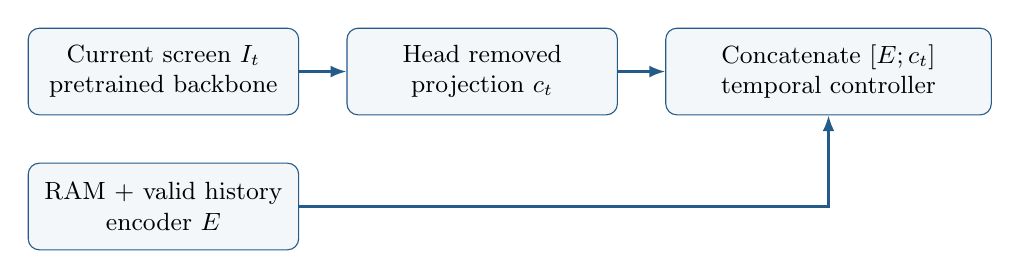
\begin{tikzpicture}[node distance=6mm]
\node[box,text width=32mm] (im) {Current screen $I_t$\\pretrained backbone};
\node[box,text width=32mm,right=of im] (cv) {Head removed\\projection $c_t$};
\node[box,text width=32mm,below=6mm of im] (ra) {RAM + valid history\\encoder $E$};
\node[box,text width=39mm,right=of cv] (fu) {Concatenate $[E;c_t]$\\temporal controller};
\draw[arr] (im)--(cv);\draw[arr] (cv)--(fu);\draw[arr] (ra.east)-|(fu.south);
\end{tikzpicture}
\caption{Proposed CV input fusion. The removed output head contributes no pretrained task logits to the policy. No new visual model was trained for this report.}\label{fig:futurecv}
\end{figure}

\textbf{Three equal students, trained by level teachers.} The existing teachers differ in architecture, size and action vocabulary. A proposed replacement uses three copies $S_{\theta_1},S_{\theta_2},S_{\theta_3}$ of \emph{one} architecture with identical input schema and parameter count $P$ each. Copy$\ell$ learns from frozen level teacher $T_\ell$ on that level's validated inputs. Let $\mathcal A_\cup$ be the union of native controller masks; map teacher outputs by exact mask identity into a common head of width $|\mathcal A_\cup|$, with explicit level-valid masks. DQfD teacher Q values are converted to temperature-scaled soft targets; imitation teachers supply temperature-scaled logits:
\begin{equation}\label{eq:distill}
 p^T_\ell=\operatorname{softmax}(u^T_\ell/\tau),\quad
 L_\ell=\tau^2\operatorname{KL}(p^T_\ell\|p^S_\ell)+\alpha\operatorname{CE}(a_{\rm verified},p^S_\ell).
\end{equation}
Q scale and logit calibration must be checked independently; soft Q targets are a design choice, not action probabilities inherent in DQN. Common adapters and padded/masked action heads preserve equal student sizes. Teachers retain their own validated observation contracts during data generation.

Concatenate equal-width representations $h_t=[h_t^1;h_t^2;h_t^3]\in\mathbb R^{3d}$ and train a fusion head $p_F=\operatorname{softmax}(W_Fh_t+b_F)$ with balanced level replay and the active teacher's loss. Total capacity is $3P+P_F$ (plus any shared visual encoder), not $P$. Level choice must use a validated runtime transition contract, never a demonstration cursor. First establish per-level retention, then uninterrupted transitions and the official10-episode campaign. This architecture is proposed only; no training result, timing or parameter budget is claimed. Priority remains normal-start validation, independent starts and asset access before greater model complexity.

\clearpage
\appendix
\topic{APPENDIX A / REWARD CONTRACTS}{Exact scales, availability and safeguards}
\begingroup\small
The selected checkpoint's embedded config is the authority for Level~1 coefficients. Its config SHA-256 is \texttt{f2a28db6efc046b8527fab61b39a21fff2de8e3762eedc4638f0eb8e193f6d7d}. Runtime definitions are \pathref{backward_level1.TaskHistory.transition}, \pathref{Level1Env.step}, \pathref{route_guidance} and \pathref{level1_potential}. Paths are under \pathref{src/prince_valiant_rl/} unless otherwise stated. \ev{E02,E07}

\begin{table}[ht]\small\centering
\begin{tabularx}{\linewidth}{@{}P{27mm}P{15mm}Y Y@{}}\toprule
Term & Weight & Event / units & Availability, rationale and anti-farming rule\\\midrule
new\_progress & $0.2$ & $\max(0,x_{t+1}-F_s)/16$; section-local pixels & Live supported state; per-section frontier persists through death/retracing; reset past seeded unpaid.\\
checkpoint reached & $2$ & First entry to section $s>0$ & Section visited-set blocks repeated awards.\\
objective\_cleared & $3$ & First verified gate0$\to$1 & Four gate identities513--516; set survives retracing.\\
level\_completed & $40$ & Fresh verified native completion & Once per episode, not arbitrary title/flag.\\
route\_corridor & $2$ & Discounted potential difference & Pinned phase-corridor data; bootstrap/scope condition in source.\\
combat potential & $6$ & Discounted type14 potential difference & Verified encounter scope; no universal enemy HP interpretation.\\
enemy\_kills & $0.25$ & Verified observer defeat events & Native ABI diagnostics; unavailable coverage retained explicitly.\\
score\_gain & $0.00005$ & Positive valid packed-BCD score points & $\$F4$--$\$F6$ validation; reset baseline unpaid; unexplained decrease quarantined in selected policy.\\
player\_damage & $-2$ & $\max(0,H_t-H_{t+1})/255$ & Only live/live, same lives and section. Ambiguous fatal writes unavailable.\\
death\_started & $-2$ & Life phase0$\to$1 & Once on transition; distinct from life decrement.\\
lives\_lost & $-4$ & Positive signed retry decrement & Real native losses retained; reset is not a loss event.\\
game\_over & $-4$ & Fresh verified terminal & No repeated terminal charge.\\
elapsed\_seconds & $-0.03$ & $1/60$ per native frame & Actual duration charged, discouraging waiting.\\
enemy\_damage & $0$ & Unavailable generic damage & No reward; no invented semantic zero.\\
ABI2 kind18 defeat & $0$ & Optional scoped sidecar event & Disabled coefficient; not an extra unverified kill bonus.\\\bottomrule
\end{tabularx}\caption{Complete selected Level~1 reward contract. $F_s$ is the saved section frontier; $H$ is HP. Coefficient sensitivity on a saved trace is not a training ablation.}
\end{table}

\textbf{Level~2 versions and source.} \pathref{training/level2_runtime.py:transition} supplies v3: completion100, game over$-25$, ENERGY loss$-5\max(0,E_t-E_{t+1})/255$, time$-0.01d/60$; kill/progress/shot are zero. \pathref{training/level2_score_reward.py:transition} adds v4 score$0.01(S_{t+1}-S_t)$ and rejects invalid BCD/decreases. \pathref{config/level2_aim_hold_v9_20261025.json} and its owning aim modules add0.25 aim potential and0.03 aim-hold/second, under shootable/eligible scoped geometry. Hold requires distance zero before and after a nonterminal transition, paying $0.03/60$ per native frame. Those aim signals can favor proxy behavior, so old-enemy and real scoring gates remain necessary. The earlier prepared v5 temporary-removal curriculum was not automatically executed by the unchanged trainer. The final v57 actor optimizes cross-entropy, not any reward in this table.

\textbf{No Level~3 task reward is defined.} Reporting its classification accuracy as return would change the metric. Missing episode-return and completion-rate curves remain unavailable; source-fit diagnostics do not replace acceptance metrics.

\endgroup
\newpage
\topic{APPENDIX B / TRACEABILITY}{Primary artifacts and retained implementation}
\small
Evidence IDs resolve to the accompanying \pathref{evidence_ledger.csv/json}, including SHA-256, classification, experiment, reset/config/checkpoint, metric units and limits. The following paths are relative to the research root; package equivalents are inspected separately.

\begin{tabularx}{\linewidth}{@{}P{15mm}Y@{}}\toprule
ID & Primary artifact and precise role\\\midrule
E01 & \pathref{src/prince_valiant_rl/recorder_native.py}: \texttt{RecorderNative}, \texttt{dump\_state}, \texttt{load\_state}; C ABI in \pathref{instrumentation/recorder_api.cpp}.\\
E02--03 & \pathref{analysis/level1_dqfd_demo_continuation_20261025/selected_checkpoint.json}, \texttt{result.json}; \texttt{episodes}, \texttt{candidate\_comparison}, \texttt{phase\_complete\_payload}. Committed checkpoint receipts in corresponding \pathref{training/} directory.\\
E04--06 & \pathref{src/prince_valiant_rl/training/dqfd.py}: \texttt{paired\_return}, \texttt{paired\_targets}, \texttt{dqfd\_objective}; \texttt{dqfd\_execution.py}: \texttt{update}; \texttt{dqn.py}: \texttt{DuelingQ}; \texttt{temporal\_models.py}: \texttt{WindowPath}.\\
E07--08 & \pathref{src/prince_valiant_rl/backward_level1.py}: \texttt{TaskHistory}, \texttt{Level1Env}; \pathref{docs/REA_OBSERVATION_AUDIT.md}; executed/ROM identity records under \pathref{analysis/rea_audit/}, including \texttt{rea\_*.json} and \texttt{rom\_identity.json}.\\
E09 & \pathref{analysis/level1_full_route_verification_20261023/}: \texttt{result.json}, \texttt{fit\_audit.json}, \texttt{evaluation\_summary\_recovered.json}; original aggregate report failure preserved.\\
E10--11 & \pathref{analysis/level1_demo_bc_ppo_aux_comparison_20261022/README.md}; allocator sizes and skipped fixed reviews; \pathref{analysis/level1_anchored_ppo_earlier_17760_20261023/README.md}; endpoint/reset hashes and exact production trace paths.\\
E12--13 & \pathref{training/level2_expanded_drop_adapter_v33_20261025/}: \texttt{result.json}, \texttt{diagnostics.jsonl}; \pathref{analysis/level2_drop_objective_conflict_v36_20261026_v2/audit.json}: \texttt{checkpoints}, \texttt{paired\_trials}, gradient norms/cosines/delta products.\\
E14--16 & \pathref{analysis/level2_drop_dispatch_v50_20261026/README.md}; \pathref{training/level2_motion_study_v51_20261026/result.json}; \pathref{analysis/level2_matched_spawn_pickup_v53_20261026/README.md}.\\
E17--18 & \pathref{training/level2_title_bc_v57_20261026/result.json}; \pathref{analysis/level2_transition_tail_v59_20261026/verification.json}; \texttt{E\_collections}, \texttt{T\_collections}, \texttt{missed\_opportunities}, visible card/title/gameplay fields.\\
E19--22 & \pathref{src/prince_valiant_rl/training/level3_imitation.py}; \pathref{training/level3_imitation_v1_20261026/} and \pathref{training/level3_imitation_refine_v2_20261026/}: \texttt{fit.jsonl}, \texttt{result.json}; \pathref{analysis/level3_imitation_evaluation_v2_20261026/verification.json}.\\
E23--24 & \pathref{../github_submission/prince-valiant-rl/manifests/}: inventory, artifacts, provenance, dependency graph and verification JSON; \pathref{../submission_demo_videos/manifest.json}.\\\bottomrule
\end{tabularx}

\textbf{Packaged runtime closure.} DQfD preparation imports the lazy \pathref{dqfd_level1_adapter}, then \pathref{HumanRoute/Level1Env}; runtime data include route JSON/NPZ/states and paired-return cache manifest/READY/identity/windows. PPO imports \texttt{process\_envs}, \texttt{level1\_child}, control/window history and the same schema-specific encoders. Level~2 fitting depends on v4 replay, immutable SQLite labels, title intro/reset and v56 parent; completion imports \texttt{CompletionEvidence}. Level~3 preparation uses segmentation/index/SQLite; fit consumes selected ancestry; evaluation needs checkpoint, preparation metadata, reset, ROM and DLL; independent review additionally needs saved actions/RAM and terminal references. The general environment requires its separate \texttt{nes\_py} and gameplay state assets.

\textbf{Package review receipts.} \pathref{packaged_source_inventory.json} enumerates actual packaged symbols, line numbers and imports. \pathref{evidence_verification.json} records inventory hash and dependency-file checks. Existing verification covers CLI help, static compilation, isolated staged imports and CPU checkpoint shape/hash checks. It explicitly records no native load/training/gameplay or clean-machine installation. Static closure cannot supply absent runtime artifacts or certify state compatibility.

\newpage
\topic{APPENDIX C / PROTOCOL DETAILS}{PPO, runtime identities and reporting limits}
\textbf{Observed PPO evidence and testable hypotheses.}\par
{\small
\begin{tabularx}{\linewidth}{@{}P{38mm}Y Y@{}}\toprule
Observed evidence & Plausible mechanism / alternative & Discriminating future test\\\midrule
Anchored endpoints at reset17760 die at 3,971/3,421 frames, returns $-38.0815/-38.1789$; first action divergence after 4/5 decisions. & Coverage mismatch or brittle timing; alternatively insufficient optimization of the local start. & Matched earlier-start exposure with fixed rewards, seeds and held-action interval.\\
Critic calibration guide reports large fresh-return errors; control timing changes alter suffix results. & Value instability and precise edges are relevant; different trajectory distributions also change error. & Fixed-policy evaluation set, critic-only fit, then matched PPO continuation.\\
BC-aux pilot stops at 37 vs2 completed cycles from host allocation failures; scheduled reviews never reached. & Infrastructure limits exposure; it is not evidence that either objective is worse. & Resume only under a new declared protocol with preserved rollout semantics and equal budgets.\\\bottomrule
\end{tabularx}}
\medskip
\textbf{Standard explanatory PPO equations.} With behavior policy $\pi_{\rm old}$, $r_t^\pi=\pi_\theta(a_t\mid W_t)/\pi_{\rm old}(a_t\mid W_t)$, clipping $\epsilon$, and advantage $\hat A_t$, the surrogate is \cite{ppo}
\begin{equation}
 L^{\rm clip}=\mathbb E\left[\min\{r_t^\pi\hat A_t,\operatorname{clip}(r_t^\pi,1-\epsilon,1+\epsilon)\hat A_t\}\right].
\end{equation}
The project trains separate actor/critic paths with value regression and entropy terms; optional human auxiliary cross-entropy is configuration-dependent. This equation is explanatory, not a claim that all historical variants use identical total-loss weights. GAE with duration-aware continuation can be written
\begin{equation}
 \delta_t=r_t+\gamma^{d_t}b_tV(W_{t+1})-V(W_t),\qquad
 \hat A_t=\delta_t+(\gamma\lambda)^{d_t}c_t\hat A_{t+1}.
\end{equation}
Bootstrap flag $b_t$ and recursion/episode flag $c_t$ have different purposes: a time limit can bootstrap the actual next observation while stopping aggregation across the following reset. In selected skip1 configurations $d_t=1$. Exact rollout/GAE implementation is in \pathref{scripts/train_backward_level1.py:optimize/main} and temporal storage helpers; reconstructing a policy input must preserve reset masks and actual executed controls.

\textbf{Exploration and accounting.} The offline Level~1 continuation applies 3,000 updates from global2,001 through5,000, draws384,000 row presentations, uses fixed PER beta0.6, and has no epsilon exploration phase. Its three greedy evaluations total63,792 native frames. Earlier PPO's constant entropy0.0002 is not entropy decay; epsilon0.03$\to$0.01 is its configured collection mixture, not evidence of a measured convergence transition. Supervised Level~2/3 fitting has no environment exploration schedule. Episode-return points in Figure~\ref{fig:l1}, score gains in the extended development plot, and cross-entropy in Figure~\ref{fig:l3fit} have different units and cannot form a common learning curve.

\newpage
\topic{APPENDIX C / COMPUTE AND IDENTITIES}{Measured phase costs and selected checkpoints}
\textbf{Compute.} Recorded hardware is RTX 4060 Laptop GPU (about 8GiB VRAM), Python 3.13.1, PyTorch 2.14.1+cu130/CUDA 13.0. Level~3 fit times are 38.920915 and 47.254369 seconds: 86.175284 seconds subtotal. Level~1 continuation's whole command is 1,353.622729 seconds, including model-I/O/setup and demonstrations/encoding; it applies 3,000 new updates and 63,792 native evaluation frames. Its 600-second preparation debit is an allowance, not measured training. Whole-project compute/development time cannot be reconstructed. The assignment's13.10.2026 prose and 16.10.2026 table conflict; no extension is inferred.


\textbf{Level2 staged learning.} In the three-encounter study, reward-only v13 applied 1,500 updates without a shared aim pass; geometry-guided v14 passed individual stages but forgot earlier cases. V15 adds agent-state rehearsal: aim uses geometry cross-entropy plus L2, and shooting uses paired TD with directional cross-entropy. It is mixed supervision, not pure RL or human cloning. Shared gates pass aim at 300 and shooting at 700 updates; 147 remaining catalogue encounters were not trained. Earlier-start expansion and self-imitation did not establish full-route mastery. \pathref{analysis/level2_encounter_curriculum_v13_20261025/README.md} records action masks, gamma 0.99 and exact gates.

\textbf{Original backward PPO protocol.} The first backward experiment used fresh actor/critic weights, no BC, history offsets$[-10,-5,0]$, six CPU owners,256 decisions/owner, minibatches256, three PPO epochs, clip0.2, actor LR$10^{-4}$, critic LR$3\times10^{-4}$, entropy0.01, $\gamma=0.9999$, $\lambda=0.97$. It began at route frame18302; at least20 frontier episodes in a40-episode window with20\% completions moved the frontier300 frames earlier. This differs from the later seven-history recovery lineage. \pathref{docs/BACKWARD_LEVEL1.md} records these original contracts.

\textbf{Reward evolution.} Original Level1 v1 used progress0.05, first section1, objective3, completion20, HP fraction$-2$, death$-2$, life$-4$, time$-0.01$/second and game over$-4$; kills/damage/score were unavailable with zero coefficients. The later selected v6 adds corridor/combat shaping and validated score/defeat events (Appendix~A), increases completion to40 and progress to0.2, and raises time cost to$-0.03$/second. These are documented revisions, not a controlled one-factor ablation.

\textbf{Selected identities (full SHA-256).}\\
Level~1 \pathref{training/level1_dqfd_demo_continuation_20261025/checkpoint_3000.pt}\\
\pathref{7e44f1bc067b8cb827dfa8594a15fe7a7a51896a7bf0ab9ff104977c6f97d7c6}\\
Level~2 \pathref{training/level2_title_bc_v57_20261026/actor.pt}\\
\pathref{900c098cbe0376cfbc5aabc4c145b83fcd96b377772c6528e1a42beb9e9efbbd}\\
Level~3 \pathref{training/level3_imitation_refine_v2_20261026/best.pt}\\
\pathref{1481dd27a35a04e97bcb9dd25717171d16d25fa9063e18cda69e404f9f5afbcb}\\
Level~1 route hash\\
\pathref{214b5d56f858a45690779c11441ee3251880a1e8bf3418e564f461fe655b6eed}

\textbf{Historical discrepancies retained.} The epoch400 README contains a stray ``Prince of Persia'' environment label; the game/ROM/route identity is Prince Valiant. The old v5 handoff's ``no learned completion'' and older video/report status are superseded only by scoped later artifacts, not erased. Eight mixed-start BC evaluations are not eight normal-start trials. A single milestone's binary completion is not a reliable100\% success rate. Source-correlated timing variants receive no independent-trial confidence intervals. Classification agreement uses the full training route. Missing total-project compute, reward-rate curves and clean-machine runs are not reconstructed from budget ceilings.

\textbf{Build scope.} This PDF and all figures are generated without game execution. The LaTeX source, bibliography, plotted CSVs, source hashes and read-only audit scripts accompany it. No matching DOCX is supplied: preserving these equations, diagrams and cross-references through the available conversion path has not been visually validated in Word. The original editable draft remains preserved separately.

\newpage
\topic{APPENDIX D / EXTENDED FIGURES}{Transfer, interference and continuous-route development}
\fig{08_gradient_conflict.pdf}{.73}{v36-v2 fixed-dataset diagnostics at v35 updates0/25. Negative cosines identify opposing parameter gradients; they do not reproduce stochastic Adam updates. CSV: \texttt{gradient\_cosines.csv}. Source: E13.}{fig:gradient}
\fig{03_timing_transfer_and_limit.pdf}{.72}{v51 matched familiar timing gains do not extend to the reserved cases. Counts are correlated reset probes, without independence-based error bars. Source: E15.}{fig:transfer}
\fig{05_full_run_development.pdf}{.82}{Continuous Level~2 development attempts have different starts/supervision/controllers. Game score is not RL return; historical clear flags are corroborated later by v59. This is descriptive development evidence, not an algorithm ablation. Source: v54--v57 result JSON.}{fig:fullroute}

\clearpage
\topic{APPENDIX E / REFERENCES AND PROPOSED SCHEMA}{Algorithm sources and the concatenated student design}
\textbf{Proposed student tensor schema.} Each of three equal-size students receives the same adapter-defined observation contract: current/past RAM $[K,2048]$ plus validity $[K,1]$, and optionally aligned visual features $[K,d_c]$. A fixed common $K$, feature width and common action vocabulary preserve identical architecture and parameter count. This schema is a proposal; it is not retroactively attributed to the existing level teachers. A minimal first experiment could use $K=1$; temporal variants require a newly validated history/reset contract.

\begin{figure}[ht]\centering
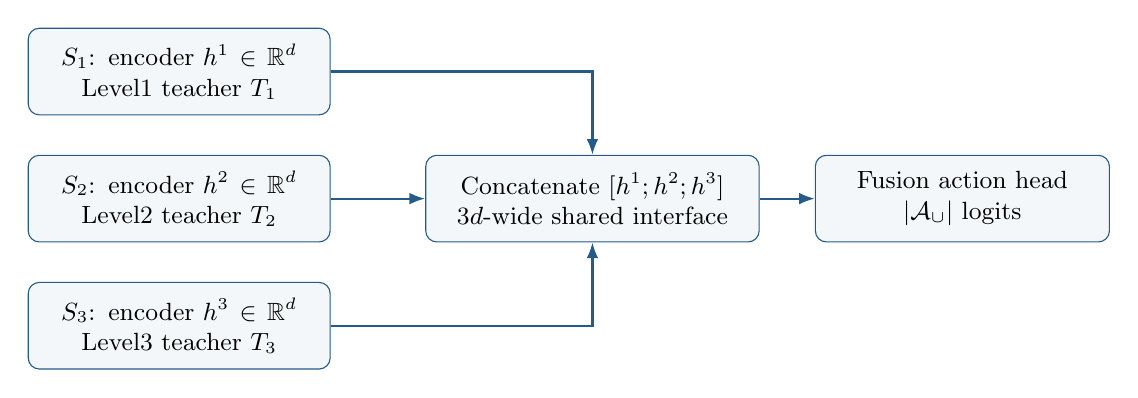
\begin{tikzpicture}[node distance=5mm]
\node[box,text width=36mm] (s1) {$S_1$: encoder $h^1\in\mathbb R^d$\\Level1 teacher $T_1$};
\node[box,text width=36mm,below=of s1] (s2) {$S_2$: encoder $h^2\in\mathbb R^d$\\Level2 teacher $T_2$};
\node[box,text width=36mm,below=of s2] (s3) {$S_3$: encoder $h^3\in\mathbb R^d$\\Level3 teacher $T_3$};
\node[box,text width=40mm,right=12mm of s2] (cat) {Concatenate $[h^1;h^2;h^3]$\\$3d$-wide shared interface};
\node[box,text width=35mm,right=7mm of cat] (out) {Fusion action head\\$|\mathcal A_\cup|$ logits};
\draw[arr] (s1.east)-|(cat.north);\draw[arr] (s2)--(cat);\draw[arr] (s3.east)-|(cat.south);\draw[arr] (cat)--(out);
\end{tikzpicture}
\caption{Proposed equal-architecture students and concatenated fusion, requested as future work. Train level specialists with mapped teacher targets, then fusion with balanced replay and retention gates. Three encoders increase total capacity and inference cost.}\label{fig:students}
\end{figure}

For level-balanced batches $D_1,D_2,D_3$, a possible fusion objective is
\begin{equation}
 L_F=\frac13\sum_{\ell=1}^3\mathbb E_{(o,a)\sim D_\ell}
 \left[\tau^2\operatorname{KL}(p^T_\ell(o)\|p_F(o))+\alpha\operatorname{CE}(a,p_F(o))\right].
\end{equation}
This explicitly labels a future loss, rather than claiming it exists in the repository. Begin with frozen specialist encoders so fusion can be diagnosed independently; test joint fine-tuning only with old-level action and completion gates. Teachers must label the actual visited states or be restricted to verified data coverage. Distillation cannot manufacture a recovery skill absent from every teacher. Evaluate concatenation against three separately deployed equal students and a single matched-budget student; report native frames, parameters, latency, per-level returns/lengths and official completion counts. No such experiment has yet been run.

\bibliographystyle{plain}
\bibliography{references}

\clearpage
\topic{APPENDIX F / IMPLEMENTATION DETAILS}{Tensor schema, replay settings and diagnostics}
\small
\textbf{Selected Level1 per-timestamp schema.} The main-text architecture groups resolve to the following checkpoint-specific tensors. No other experiment's features are blended into these shapes.

\begin{tabularx}{\linewidth}{@{}P{39mm}P{29mm}Y@{}}\toprule
Selected Level~1 per timestamp & Shape & Representation / constraint\\\midrule
Scalars; categorical & 61; 21 & Fixed scales; categorical byte embedding dimension~3\\
Entities; codes & $10\!\times\!11$; $10\!\times\!9$ & Relative geometry, continuity/occupancy masks and raw codes\\
Projectiles; codes & $3\!\times\!4$; $3\!\times\!3$ & Scoped active/flying masks; raw direction/state\\
Triggers; codes & $16\!\times\!5$ each & ROM trigger rectangles; validity; not sprite hitboxes\\
Tiles; classes; terrain validity & $12\!\times\!17$ each & Two embeddings dimension~4; unknown code~256\\
Dynamic actors; rope points & $12\!\times\!17\!\times\!11$; $12\!\times\!17\!\times\!9$ & Moving geometry supplements static terrain\\
Resident codes; validity & $25\!\times\!11$; $25\!\times\!1$ & Masked resident records; schema \texttt{rea\_expanded\_v2}\\\bottomrule
\end{tabularx}

The continuation samples $B=128$ rows with replacement. Its base priority is $p_i=\max(|\delta_i^{(1)}|,|\delta_i^{(10)}|)+0.001$, with duplicate samples aggregated by maximum error; demonstration sampling mass adds~1:
\begin{equation}
 P(i)=\frac{(p_i+1)^{0.4}}{\sum_j(p_j+1)^{0.4}},\qquad
 w_i=\frac{(N P(i))^{-0.6}}{\max_{j\in\text{sample}}(NP(j))^{-0.6}}.\label{eq:per}
\end{equation}
Adam uses $10^{-4}$, $(\beta_1,\beta_2)=(0.9,0.999)$, $\epsilon=10^{-8}$, zero optimizer weight decay and gradient clipping at 10. Target copies occur every 1,000 successful global updates. The continuation restores Q, target, Adam, RNG and PER from the committed update-2,000 state; it does not restart a new optimizer or collect online replay. \ev{E02--E05} Prioritized replay is motivated by \cite{per}; this experiment's fixed $\beta=0.6$ is not an annealed exploration schedule.


\textbf{PPO conditions and negative evidence.} The selected lineage's temporal actor and critic are independent. A representative recovery config uses six owners, $2048$ rollout decisions each, three PPO epochs, minibatches~512, actor LR $10^{-5}$, critic LR $3\times10^{-4}$, clip~0.1, $\gamma=0.99997$, $\lambda=0.9995$, and constant entropy coefficient 0.0002. Its historical epsilon schedule is 0.03 to 0.01 over 250,000 frames; those settings belong to PPO collection, not the offline DQfD continuation. The standard explanatory PPO/GAE equations appear in Appendix~C. \ev{E02,E10,E11}


\textbf{Level3 fitting settings.} Initial fitting applied 20,000 updates at initial LR$10^{-3}$. Refinement applied 15,500 with a fresh Adam optimizer and initial LR$10^{-5}$; it is supervised continuation, not an executed failed RL experiment. Batches have 1,024 rows; after 3,000 initial updates (immediately on resume), half are sampled from current errors. Learning rates multiply by~0.3 at local updates 5,000/10,000/15,000. Gradient norm clips at~10. The recorded seed is 20261130. \ev{E20,E21}


\textbf{Interference diagnosis.} In v35, balanced data and soft successful-action rehearsal still forgot two timing variants at start~15211 after 25 updates, so the candidate was rejected. At shared pre-action RAM, fire+right (mask129) changed to down (mask32). Successful-action margins reversed from $+0.014011$ to $-0.002201$ and $+0.008785$ to $-0.003607$. The fixed-dataset diagnostics are
\begin{equation}\label{eq:interference}
 c_{uv}=\frac{\nabla L_u\cdot\nabla L_v}{\|\nabla L_u\|\|\nabla L_v\|},\quad
 M(s)=Q(s,a_{\rm success})-Q(s,a_{\rm replacement}).
\end{equation}
TD/rehearsal cosine is $-0.5671$ initially and $-0.4918$ at update25; geometry/rehearsal is $-0.4956$ and $-0.6216$. Geometry merges fire/NOOP and fire/horizontal actions by direction, providing no fire label. Rehearsal is a weighted penalty, not a preservation constraint. Aggregate rehearsal gradients can reduce the vulnerable margin despite including that action's label. Minibatch sampling, weighting and Adam momentum prevent causal reconstruction of the real update path from these first-order measurements. \ev{E13}


\textbf{Curriculum configuration.} The later selected lineage records a 60-episode advancement window, at least 40 episodes, a 0.2 success threshold, 120-frame earlier steps and 30-frame refinement near the ending. The ordered-fixes collector layout used one full-start, one coverage and four frontier/rehearsal owners; later configs differ. These are rules and attempted exposure, not evidence that every frontier was mastered.

\textbf{Terminal-reference check.} Active rendering avoids stale framebuffers. Title matching uses exact RGB under a validated $\pm4$-pixel shift (observed2 pixels); the original fixed-position rejection remains preserved. \ev{E22}

\clearpage
\topic{APPENDIX F / REWARD CONTRIBUTIONS}{Observed scales, not a reward ablation}
\small
The clear column is the saved \texttt{original\_389} training trajectory in \pathref{analysis/level1_dqfd_demo_continuation_20261025/reward_sensitivity.json}; it is not newly decomposed update3000 policy telemetry. Its total matches the selected clear return, but that alone does not prove identical per-component policy totals. The failure column is anchored PPO endpoint seed1 from \pathref{analysis/level1_anchored_ppo_earlier_17760_20261023/result.json}. Both are saved configured rewards; starts and trajectories differ, so this is a scale illustration, not causal PPO/DQfD evidence.

\begin{table}[ht]\centering
\begin{tabular}{@{}lrr@{}}\toprule
Weighted contribution & Clear trace, reset389 & Failed PPO suffix, reset17760\\\midrule
First progress & 59.687500 & 0\\
Completion & 40.000000 & 0\\
Objectives & 12.000000 & 0\\
Section/checkpoint & 4.000000 & 0\\
Verified enemy defeats & 2.000000 & 0\\
Score & 0.570700 & 0.007500\\
Route corridor & 0 & 0.008618\\
Combat potential & $-0.151478$ & $-2.355300$\\
Player damage & $-0.878431$ & unavailable\\
Elapsed time & $-9.136500$ & $-1.985500$\\
Death started & 0 & $-8.000000$\\
Lives lost & 0 & $-20.000000$\\
Game over & 0 & $-4.000000$\\\midrule
Available component subtotal & 108.091791 & $-36.324683$\\
Reported undiscounted return & 108.091791 & $-38.081545$\\\bottomrule
\end{tabular}
\caption{Illustrative saved components. The failed endpoint's reported total is addressed below; unavailable events are not measured zeros. CSV: \texttt{reward\_component\_examples.csv}.}\label{tab:components}
\end{table}

The clear components sum to the recorded return. For the failure, the difference between available subtotal and reported return is$-1.756863$, exactly the raw evaluator's legacy player-damage contribution. The complete raw arithmetic reconciles, but the conservative review marks that damage quantity unavailable, so it cannot be presented as verified damage. The table therefore separates available components from the recorded return instead of silently filling unavailable semantics. Both checks are preserved in \pathref{reward_component_verification.json}. The narrower supported observation is that the verified life/death costs are substantial; the table is not a complete verified semantic decomposition of the failure.

\clearpage
\topic{APPENDIX G / REVIEWER EXECUTION}{Commands, dependencies and acceptance}
\small
From the staged package root, after installing its pinned dependencies, model inspection can run without the game assets:
\begin{quote}\ttfamily
python run.py inspect\_models\\
python run.py submission\_assets audit
\end{quote}
These were historically checked in the developer's environment, not on a clean machine. For selected evaluation, the documented commands below require the withheld assets first; they were not executed for this revision:
\begin{quote}\ttfamily\small\raggedright
python run.py evaluate\_selected\_level1 \textasciigrave{}\\
\quad -{}-output analysis/reviewer\_l1\par\medskip
python run.py evaluate\_level2\_confirmed\_completion \textasciigrave{}\\
\quad -{}-output analysis/reviewer\_l2\par\medskip
python run.py evaluate\_level3\_imitation \textasciigrave{}\\
\quad -{}-checkpoint training/level3\_imitation\_refine\_v2\_20261026/best.pt \textasciigrave{}\\
\quad -{}-output analysis/reviewer\_l3\par\medskip
python run.py review\_level3\_imitation -{}-output analysis/reviewer\_l3
\end{quote}
The backticks above are PowerShell line continuations; the same commands are copyable in \pathref{REVIEWER_COMMANDS.md}.
Level1 requires the route JSON/NPZ/state tree and exact recorded native/observer identities. Level2 requires title/preparation and initial-state files; fitting additionally needs v4 replay, immutable SQLite labels and the v56 parent. Level3 inference requires the frame44700 reset and preparation metadata; fitting/review additionally needs selected-ancestry data and actively rendered terminal references. \pathref{manifests/artifacts.json} gives exact filenames, hashes and restoration destinations. No public download links are available. Private owner access could address missing files if permitted, but licensing and build/state compatibility still need separate resolution.

\begin{tabularx}{\linewidth}{@{}P{44mm}Y P{32mm}@{}}\toprule
Assignment criterion & Evidence & Gap / status\\\midrule
Levels1--3, each at least7/10 & Known-route DQfD / imitation clears & Campaign absent\\
Deterministic/low-temperature & Greedy selected runs; frozen actors & Qualifying campaign pending\\
Level1 normal game start & Verified saved reset389 & Compliance unaudited\\
Training saves; imitation/curricula disclosed & Separate models, ancestry and reset contracts & Disclosed here\\
No evaluation life/invincibility/skip manipulation & Selected continuous ordinary-input runs; diagnostics separated & No general acceptance certification\\
Code, configs, seeds, models and logs & Curated package + pinned artifacts & Private data/native gaps\\
5--10-page PDF plus appendices & Ten main pages + technical appendices & Case study prepared\\
3--5min MP4,720p+, progression & Current 250.60s,1280$\times$960,30fps presentation and three 1$\times$ companions & Full-run interpretation; L3 reward absent\\
Private Git access and one submission link & Public GitHub repository published & Private-access requirement unresolved\\\bottomrule
\end{tabularx}

\textbf{Next validation order.} Restore compatible assets, audit Level1 normal-start compliance, and retain every outcome of the official ten-episode protocol. Test independent starts/recovery separately; correlated row splits do not establish generalization. Matched algorithm comparisons and new fusion models follow these baselines.

\end{document}
